% Conference draft v7, two stories from one source (24 November 2026).
%   draft-A.pdf  receiver story: the map and how the receiver uses it
%   draft-C.pdf  both stories: the DMRS residual first, then the receiver
% Build: ./build.sh   (text that only draft C has is printed in teal)
% Every number comes from docs/results.md, sections 1, 17, 18 and 22, and was checked against it
% by an independent audit. Red notes mark what still needs a source. Hopping is left out.

\newif\ifstoryC
\ifdefined\storyA \storyCfalse \else \storyCtrue \fi

\documentclass[conference]{IEEEtran}
\usepackage[utf8]{inputenc}
\usepackage[T1]{fontenc}
\usepackage{amsmath,amssymb,amsthm}
\usepackage{graphicx}
\usepackage{booktabs}
\usepackage{xcolor}
\usepackage{tikz}
\usetikzlibrary{positioning,arrows.meta,fit}
\usepackage{cite}
\usepackage{siunitx}
\usepackage{comment}
\usepackage{url}

\graphicspath{{figures/}}
\definecolor{Conly}{HTML}{006D6F}
\newcommand{\note}[1]{{\color{red}\footnotesize[#1]}}
% Text that only draft C has, in teal so the two drafts are easy to compare. Draft A drops it.
\ifstoryC
  \newenvironment{conly}{\par\color{Conly}}{\par}
\else
  \excludecomment{conly}
\fi
\newcommand{\C}[1]{\ifstoryC{\color{Conly}#1}\fi}
\newcommand{\Pperp}{\mathbf{P}^{\perp}}
\newcommand{\tr}{\operatorname{tr}}
\newtheorem{proposition}{Proposition}

\begin{document}

\ifstoryC
\title{Locating Selective Jamming in the 5G NR Uplink\\with the DMRS Residual, and Decoding Through It}
\else
\title{Decoding Through Selective Jamming in the 5G NR Uplink with a Learned Jamming Map}
\fi
\author{\IEEEauthorblockN{Erhan Karakoca}\IEEEauthorblockA{Bo\u{g}azi\c{c}i University, Istanbul, Turkey}}
\maketitle

\begin{abstract}
A jammer that knows where the 5G NR uplink places its reference signals can disrupt decoding at
low power by hitting only the DMRS or a few resource blocks.
\ifstoryC
Weak pilot jamming is hard to locate. Its power hides in the channel's fading, and the error
it causes appears on data symbols the jammer never touched. We use a DMRS residual that removes
from the pilot estimates the delay subspace of channels with delays up to 3\,\textmu s, so that
mainly noise and jamming remain. With known noise power, its false-alarm rate per resource block
depends only on the allocation, so its threshold needs no training data. A small network fuses
the residual with power and EVM into a map of the attacked cells. In a PUSCH link simulation with
3GPP TDL channels and a 1\% false-alarm rate, the residual raises the detection probability of
pilot jamming 15\,dB below the signal from 0.39 to 0.57. A receiver that uses the map in two
standard steps lowers the block error rate under data jamming 9\,dB above the signal from 81\% to
0.04\% on a TDL-C channel, the value a receiver given the true map also reaches.
\else
A standard receiver assumes that only noise impairs each resource element, so it decodes jammed
symbols as if they were clean. We let the receiver estimate a map of the attacked cells from its
own signals with a small network and use the map in two standard steps. Pilots of flagged
resource blocks get less weight in the channel interpolation, and the estimated jamming power is
added to the noise variance of flagged data cells. In a PUSCH link simulation on a TDL-C channel
at 15\,dB SNR, with a jammer on 4 of 12 scheduled resource blocks 9\,dB above the signal, the
block error rate under data jamming falls from 81\% to 0.04\%, the value a receiver given the true
map also reaches, while a power-test map used by erasure leaves 19\%. With the noise power
estimated in every slot, the block error rate stays at or below 0.23\% in these tests.
\fi
\end{abstract}

% ---------------------------------------------------------------------------------------------
\section{Introduction}

The 5G NR uplink carries each user's data in the resource blocks the base station schedules,
with demodulation reference signals (DMRS) at fixed, published positions~\cite{gpp20265g}. A
jammer that knows these positions can hit only the DMRS or only some resource
blocks~\cite{clancy2011efficient,lichtman20185g}. In our simulation, pilot jamming reaches 50\%
block error rate with 4--5\,dB less jammer energy than data or partial-band jamming. Such attacks
are practical. A compromised user equipment (UE) can learn the uplink grants and aim noise bursts
at a target user's allocation~\cite{alaimo2025exploiting,alaimo2026when}.

A standard receiver estimates the channel from the DMRS and assumes that only noise impairs each
resource element. Jammed pilots corrupt the channel estimate of their resource blocks, and jammed
data symbols are decoded as if they were clean. The decoder then receives wrong bits that it
trusts, and the block can fail its CRC.

Li et al.\ detect corrupted tones with a power test, drop the corrupted pilots and adapt the
log-likelihood ratio (LLR) rules~\cite{li2012robust}. \"Ornek and Kartal map the error vector
magnitude (EVM) per symbol and resource block~\cite{ornek2024advanced}. Mehrabian and Kaddoum
project the pilot-period samples of several antennas onto the orthogonal complement of the known
pilot sequence and test the energy that remains~\cite{mehrabian2026robust}. Residuals of pilot
estimates outside the channel's delay span are also used for noise estimation in DFT-based channel
estimation and for jamming estimation in a patent application \note{add citations: Nguyen 2007,
Sheng 2014, Zhong WO2022151467A1}. Learned receivers already combine pilot and data observations on
the NR resource grid~\cite{honkala2021deeprx}.

\begin{conly}
Weak pilot jamming is the hard case for power and EVM tests. At 15\,dB below the signal, a per-cell
power test finds 1\% of the jammed pilot cells and an EVM test none. The jammer adds a few percent
to the power of a DMRS cell, which the channel's fading hides, and its effect on EVM appears on the
data symbols of the attacked resource blocks, which the jammer never touched (Fig.~\ref{fig:attacks}a).
The jammer has to be found on the DMRS itself.
\end{conly}

This paper makes three contributions.
\begin{itemize}
\ifstoryC
\item {\color{Conly}We derive the false-alarm law of a per-PRB DMRS residual built on a uniform
  delay subspace. With known noise power and the channel inside the retained subspace, it depends
  only on the allocation, and the link simulation confirms it.}
\item We fuse power, EVM and the residual in a small U-Net that maps the attacked cells of a slot,
  placing pilot attacks on the DMRS cells although their EVM damage appears elsewhere. The residual
  raises the detection probability of weak pilot jamming by 0.18.
\item We use the map in a standard receiver in two steps. At the tested point its block error rate
  shows no significant difference from a receiver given the true map, where a per-cell
  power-test map used by erasure leaves up to 29\%.
\else
\item A map of the attacked cells of each slot, estimated by a small network from the receiver's
  own power, EVM and DMRS observations. It places pilot attacks on the DMRS cells although their
  EVM damage appears elsewhere.
\item Two standard receiver steps that use the map softly. Pilots of flagged resource blocks are
  down-weighted in the channel interpolation, and the estimated jamming power is added to the
  noise variance of flagged data cells.
\item A PUSCH link evaluation in which the receiver shows no significant difference from a
  receiver given the true map, also with estimated noise power, where a per-cell power-test map
  used by erasure leaves up to 29\%.
\fi
\end{itemize}

% ---------------------------------------------------------------------------------------------
\section{System Model}

We consider one PUSCH slot of 14 OFDM symbols on a carrier of 24 resource blocks (PRBs) with
30\,kHz subcarrier spacing. The UE has one antenna, one layer and QPSK with LDPC coding, on a
contiguous allocation of $n \ge 6$ PRBs. One DMRS symbol (symbol 2) carries pilots on every second
subcarrier, so the allocation has $N = 6n$ pilots. The base station (gNB) has one antenna. The
received value on subcarrier $k$ of symbol $l$ is
\begin{equation}
  y_{k,l} = h_{k,l}\, x_{k,l} + g_{k,l}\, z_{k,l} + w_{k,l},
  \label{eq:model}
\end{equation}
where $h$ and $g$ are the frequency responses of the UE's and the jammer's 3GPP TDL
channels~\cite{3gpp38901}, $x$ is the UE's symbol, $z \sim \mathcal{CN}(0, S_J)$ the jamming
signal and $w \sim \mathcal{CN}(0, N_0)$ the noise.

The jammer knows the numerology, the slot timing and the DMRS position, but not the data or the
channels. It jams a block of PRBs on the DMRS symbol only (\emph{pilot}), on the 13 other symbols
(\emph{data}), or on all symbols (\emph{partial-band}), as in Fig.~\ref{fig:attacks}. In the
detection data it does not know the allocation. The decoding and margin experiments place it on
scheduled PRBs. Its strength is the jammer-to-signal ratio (JSR) per jammed resource element,
relative to the UE's energy per data resource element. DMRS resource elements carry 3\,dB more. We
call one PRB on one OFDM symbol a \emph{cell}. The detector outputs a $24 \times 14$ map per slot,
and its label marks the cells where the jammer transmitted, not the cells whose symbols are
degraded. Table~\ref{tab:assumptions} lists the assumptions of the study and where each one is
tested.

\begin{figure}[t]
\centering
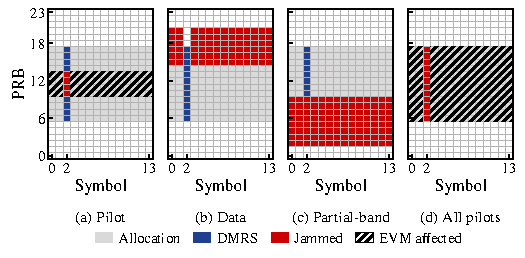
\includegraphics[width=\columnwidth]{attack_patterns.pdf}
\caption{The attacks on a slot with the UE on PRBs 6--17 and the DMRS on symbol 2. (a) Pilot
jamming of 4 PRBs, (b) data jamming of 6 PRBs, (c) partial-band jamming of 8 PRBs, (d) pilot
jamming of the whole allocation. Hatched cells are not jammed, but their EVM rises because the
jammed pilots spoil their channel estimate.}
\label{fig:attacks}
\end{figure}

\begin{table}[t]
\caption{Assumptions of the study and where each one is tested, as F1 / false-alarm rate of the
fused detector}
\label{tab:assumptions}
\centering
\footnotesize
\setlength{\tabcolsep}{3pt}
\begin{tabular}{@{}p{0.25\columnwidth}p{0.35\columnwidth}p{0.35\columnwidth}@{}}
\toprule
Assumption & When it fails & Remedy tested \\
\midrule
Channel delays below \SI{3}{\micro\second} & 1000\,ns delay spread, 0.795 / 6.7\% & training that includes such channels, 0.918 / 1.6\% \\
Known noise power & per-slot estimate given to a U-Net trained on the true value, 0.839 / 10.2\% & U-Net trained on the estimate from the empty DMRS comb, 0.948 / 0.67\% \\
Channel constant over the slot & up to 30\,m/s, 0.857 / 5.5\% & training that includes such channels, 0.947 / 1.0\% \\
UE and jammer on the slot grid & not tested & stated as a limit \\
One receive antenna & not tested & stated as a limit \\
\bottomrule
\end{tabular}
\end{table}

% ---------------------------------------------------------------------------------------------
\section{Locating the Jammed Cells}

The detector uses three features of each cell, all computed by the receiver and divided by $N_0$
(Fig.~\ref{fig:pipeline}).
\begin{itemize}
\item \emph{Power} $P$, the mean received energy of the cell, on the whole carrier. It responds to
  every attack's energy, but the UE's fading masks weak jamming.
\item \emph{EVM} $E$, the squared distance of the equalized data symbols from their nearest QPSK
  point, summed over the cell and divided by the summed noise variance of the equalizer. It sees
  jammed data, but under pilot jamming it rises on the wrong symbols (Fig.~\ref{fig:attacks}a).
\item \emph{DMRS residual} $R$, on the DMRS cell of every scheduled PRB, defined next.
\end{itemize}

\begin{figure}[t]
\centering
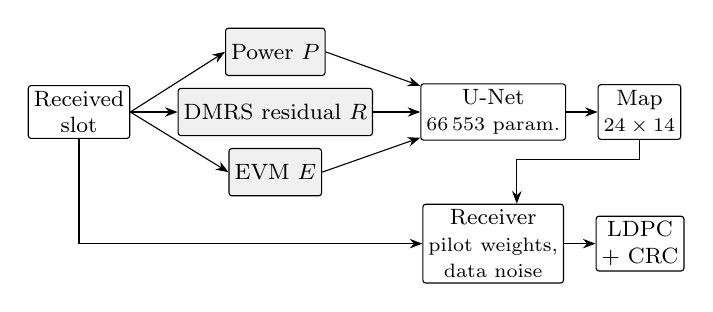
\begin{tikzpicture}[font=\footnotesize, node distance=3mm and 3mm,
  box/.style={draw, rounded corners=1pt, align=center, minimum height=6mm, inner sep=2pt},
  feat/.style={box, fill=gray!12},
  ->, >={Stealth[length=1.6mm]}]
\node[box] (y) {Received\\slot};
\node[feat, right=6mm of y] (r) {DMRS residual $R$};
\node[feat, above=1.5mm of r] (p) {Power $P$};
\node[feat, below=1.5mm of r] (e) {EVM $E$};
\node[box, right=6mm of r] (net) {U-Net\\{\scriptsize 66\,553 param.}};
\node[box, right=4mm of net] (map) {Map\\{\scriptsize $24 \times 14$}};
\node[box, below=8mm of net] (rx) {Receiver\\{\scriptsize pilot weights,}\\{\scriptsize data noise}};
\node[box, right=4mm of rx] (dec) {LDPC\\+ CRC};
\draw (y) -- (r); \draw (y.east) -- (p.west); \draw (y.east) -- (e.west);
\draw (p.east) -- (net); \draw (r) -- (net); \draw (e.east) -- (net);
\draw (net) -- (map);
\draw (map.south) -- ++(0,-2.5mm) -| ([xshift=3mm]rx.north);
\draw (y.south) |- (rx.west);
\draw (rx) -- (dec);
\end{tikzpicture}
\caption{The receiver computes three features per cell, a small U-Net turns them into a map of
the attacked cells, and the receiver uses the map to weight its pilots and to set the noise
variance of its data symbols before decoding.}
\label{fig:pipeline}
\end{figure}

\subsection{The DMRS residual}
Let $\tilde{h}_p = y_p / x_p$ be the least-squares channel estimates at the $N$ pilots. A channel
whose delays are short changes slowly from pilot to pilot, so a few patterns are enough to
describe it~\cite{edfors1998ofdm}. These patterns are the eigenvectors of the correlation matrix
$[\mathbf{C}]_{pq} = e^{-j\pi\Delta f_{pq}\tau_{\max}}\operatorname{sinc}(\Delta f_{pq}\tau_{\max})$
of a channel whose delays are spread evenly up to $\tau_{\max} = \SI{3}{\micro\second}$. We keep
the $L$ patterns that hold all but a fraction $10^{-6}$ of its energy, $L = 18$ for $n = 12$, as
the columns of $\mathbf{U}$. The residual removes them from the pilot estimates,
$\mathbf{r} = \Pperp \tilde{\mathbf{h}}$ with $\Pperp = \mathbf{I} - \mathbf{U}\mathbf{U}^H$. For a
channel with delays up to $\tau_{\max}$, what remains is essentially noise and jamming. For PRB $b$
with pilot set $\mathcal{B}$, the residual compares this remainder with what noise alone would
leave,
\begin{equation}
  R_b = \frac{\|\mathbf{r}_{\mathcal{B}}\|^2}{\sigma_p^2 \tr\big([\Pperp]_{\mathcal{B}\mathcal{B}}\big)},
  \qquad \sigma_p^2 = N_0 / P_p,
  \label{eq:residual}
\end{equation}
where $P_p$ is the pilot power. Fig.~\ref{fig:residual} shows it in one slot. Because the
residual compares the jammer with the noise and not with the UE's signal, a jammer 15\,dB below
the signal is still 5\,dB above the noise at 20\,dB SNR.

\ifstoryC
\begin{conly}
\begin{proposition}\label{prop:null}
Without jamming, with white Gaussian noise of known power $N_0$, and if the UE's channel at the
pilots lies in the span of $\mathbf{U}$,
\begin{equation}
  R_b \overset{d}{=} \sum_{i=1}^{6} \lambda_{b,i}\, \epsilon_i,
  \qquad \epsilon_i \overset{\text{i.i.d.}}{\sim} \mathrm{Exp}(1),
  \label{eq:null}
\end{equation}
where the weights $\lambda_{b,i}$ are the eigenvalues of $[\Pperp]_{\mathcal{B}\mathcal{B}}$
divided by their sum. They depend only on $n$ and on the position of PRB $b$ in the allocation.
\end{proposition}
The proof is in the appendix. Under these conditions the distribution depends on neither the
channel nor the noise power, so the threshold for a 1\% false-alarm rate follows from the
allocation alone. For $n = 12$ it ranges from 2.31 in the middle of the band to 2.56 at its edges.
Jamming of the pilots changes only the covariance of $\mathbf{r}$ for a given jammer channel.
Averaged over the jammer's fading, the same argument gives the detection probability.
Section~\ref{sec:theory} checks both against the link simulation.
\end{conly}
\else
Without jamming, with known noise power and a channel inside the retained subspace (true up to a
millionth of its energy when its delays stay within $\tau_{\max}$), $R_b$ is a weighted sum of six
unit exponentials whose weights depend only on the allocation, so its 1\%
threshold follows from theory without training data. Measured on benign test slots, the
false-alarm rate at that threshold is 1.05\% (TDL-A) and 0.95\% (TDL-C).
\fi

\begin{figure}[t]
\centering
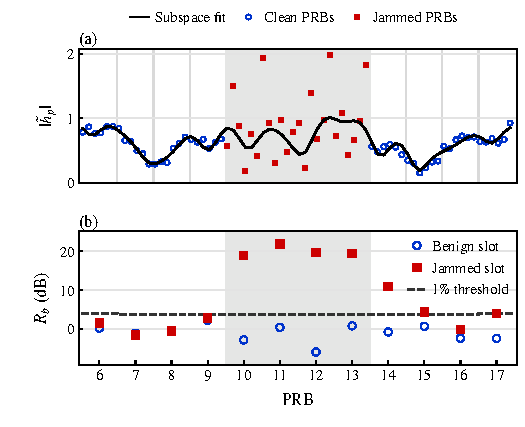
\includegraphics[width=\columnwidth]{residual_explained.pdf}
\caption{The DMRS residual in two TDL-C slots at 20\,dB SNR with the same channel and noise, one
of them with pilot jamming at 0\,dB JSR on PRBs 10--13 (shaded). (a) LS estimates at the 72
pilots of the jammed slot and their projection onto the delay subspace. On jammed PRBs the
estimates scatter around the curve. (b) Residual $R_b$ of each PRB in both slots and the analytic
1\% threshold. Leakage through the projection lifts the clean PRBs 14 and 15 above it.}
\label{fig:residual}
\end{figure}

\subsection{The map}
The three features in dB and three masks (allocation, DMRS cells, data cells) form a
$6 \times 24 \times 14$ input. A two-level U-Net~\cite{ronneberger2015unet} with 12, 24 and 48
channels (66\,553 parameters) outputs one score per cell. It is trained with a class-weighted
cross-entropy for 15 epochs on 40\,000 slots. Every detector, learned or not, is thresholded so
that it flags 1\% of the clean validation cells it scores.

% ---------------------------------------------------------------------------------------------
\section{Using the Map in the Receiver}
\label{sec:receiver}

A common use of a map is erasure. Flagged pilots are dropped and the LLRs of flagged data are set
to zero. Every false alarm then throws away clean pilots and data. Li et al.\ use a related scheme
with adapted LLR rules~\cite{li2012robust}. We use the map softly instead. It tells the receiver
where to estimate the jamming power, and the receiver lowers its trust in those cells by that
amount. Both steps below change only noise variances that an LMMSE receiver already uses.

\emph{Pilots.} The channel is interpolated by an LMMSE filter with the same delay model as the
residual,
\begin{equation}
  \hat{h}_k = \mathbf{c}_k^H (\mathbf{C} + \mathbf{D})^{-1} \tilde{\mathbf{h}},
  \qquad e_k = 1 - \mathbf{c}_k^H (\mathbf{C} + \mathbf{D})^{-1} \mathbf{c}_k,
  \label{eq:lmmse}
\end{equation}
where $\mathbf{c}_k$ is the correlation of subcarrier $k$ with the pilots and $e_k$ the error
variance of the estimate. The pilot noise $\mathbf{D} = \sigma_p^2 \operatorname{diag}(\delta_p)$
uses $\delta_p = \max(R_{b}, 1)$ for the pilots of a flagged PRB $b$ and $\delta_p = 1$ otherwise.
A strongly jammed pilot gets little weight. A falsely flagged pilot whose residual is near 1 keeps
nearly its full weight.

\emph{Data.} The jamming power on PRB $b$ is estimated from the excess energy of its flagged data
resource elements $\mathcal{F}_b$,
\begin{equation}
  \hat{S}_b = \max\Big(0,\ \frac{1}{|\mathcal{F}_b|} \sum_{(k,l) \in \mathcal{F}_b}
  \big(|y_{k,l}|^2 - |\hat{h}_k|^2 - e_k\big) - N_0 \Big),
  \label{eq:jampower}
\end{equation}
and added to their noise variance, a form of interference-aware LLR scaling~\cite{kumar2019sdr}.
The equalizer's effective noise becomes $(e_k + N_0 + \hat{S}_b)/|\hat{h}_k|^2$, which scales the
LLRs. Strong jamming drives them to zero, so the decoder treats those bits as unknown and recovers
them from the code's redundancy. After a false alarm $\hat{S}_b$ is close to zero on average, and
the cell keeps most of its weight.

% ---------------------------------------------------------------------------------------------
\section{Results}
\label{sec:results}

\subsection{Setup}
The link is simulated with Sionna~\cite{hoydis2022sionna,nvidia2026sionna} on the PyTorch backend
at 3.5\,GHz with PUSCH MCS~5 (QPSK, code rate about 0.37). Allocations of 6--24 PRBs are drawn at
random. The channels are TDL-A (100\,ns) and TDL-C (300\,ns) at up to 3\,m/s, and the SNR per data
resource element is drawn from 5--25\,dB. The channel is applied in the frequency domain, so delays
beyond the cyclic prefix cause no inter-symbol interference. Each channel draw is scaled to unit
energy over the carrier. Without that scaling the F1 score falls from 0.952 to 0.936. The jammer
hits a block of 2--12 PRBs anywhere on the carrier. Training, validation and test sets (40\,000,
5\,000 and 31\,000 slots) use separate seeds. Only 190 different allocations exist, so test
allocations repeat training ones, while channel and jammer draws do not. The test set is a grid
over channel, attack and JSR from $-15$ to $+9$\,dB in 3\,dB steps, plus 4\,000 slots without a
jammer. Each network is trained with three seeds. Detection intervals are 95\% bootstrap intervals
over batches, and paired block error rate intervals use Newcombe's method.

\ifstoryC
\begin{conly}
\subsection{The residual follows its theory}
\label{sec:theory}
Applied to every scheduled DMRS cell of the benign test slots, the analytic 1\% threshold gives
1.05\% false alarms on TDL-A and 0.95\% on TDL-C, and 0.65--1.24\% in every 2.5\,dB SNR bin
from 5 to 25\,dB. Table~\ref{tab:theory} compares the predicted detection probability with the
simulation for pilot jamming of 4 of 12 PRBs. Theory and simulation agree within 0.07, also for
the false alarms that leakage causes on the clean PRB next to the jammed block. The assumptions of
Proposition~\ref{prop:null} matter. On TDL-C with 1000\,ns delay spread, whose delays reach
8.7\,\textmu s, part of the UE's channel stays in the residual and the false-alarm rate climbs
to 62.9\%. A noise power 1\,dB too low raises it to 4.9\%, as the theory predicts (4.8\%).

\begin{table}[t]
\caption{Probability that the residual of a PRB exceeds its 1\% threshold, pilot jamming of PRBs
4--7 of a 12-PRB allocation, SNR 10\,dB, theory averaged over the jammer's fading}
\label{tab:theory}
\centering
\footnotesize
\begin{tabular}{@{}lcccc@{}}
\toprule
 & \multicolumn{3}{c}{Jammed PRB} & Clean neighbor \\
\cmidrule(lr){2-4}\cmidrule(l){5-5}
JNR & 0\,dB & 6\,dB & 12\,dB & 12\,dB \\
\midrule
Theory & 0.29 & 0.69 & 0.93 & 0.16 \\
Simulation, TDL-A & 0.30 & 0.76 & 0.94 & 0.17 \\
Simulation, TDL-C & 0.32 & 0.72 & 0.93 & 0.16 \\
\bottomrule
\end{tabular}
\end{table}
\end{conly}
\fi

\subsection{Detection}
Table~\ref{tab:detection} summarizes detection. The fused U-Net reaches an F1 score of 0.952
[0.950, 0.953] over all cells at 1.15\% false alarms. Spatial context matters more than size. A
per-cell network with about as many parameters, which sees no neighboring cells, reaches 0.707 at
its validation threshold. When each attack type gets its own matched false-alarm rate, the U-Net
still leads it by 0.096 [0.093, 0.098]. The block test, a classical detector built from the same
features with per-PRB $p$-values that are exact or calibrated on benign slots, reaches 0.868.

The residual matters for weak pilot jamming. At $-15$\,dB JSR it raises the detection probability
of jammed pilot cells from 0.39 to 0.57, a paired gain of 0.18 [0.15, 0.20].\C{ At false-alarm rates
matched per attack, the gain is 0.23 on the test set and 0.38 [0.36, 0.39] against a jammer on
exactly the scheduled PRBs.} Its effect on the overall F1 is small (0.006). Pilot cells are 1 of 14
symbols, data jamming leaves the DMRS alone, and partial-band jamming is already found on its data
symbols.
\ifstoryC
{\color{Conly}The EVM threshold scores an F1 of 0 on pilot jamming because EVM is not defined on the
DMRS symbol. It flags the data symbols of the attacked PRBs instead, cells the jammer never touched
(Fig.~\ref{fig:attacks}a). The power on the empty half of the DMRS comb finds nominal pilot jamming
better than the residual alone (pilot F1 0.721 against 0.575). A jammer that hits only the pilot
comb leaves it clean, however. Against such a jammer a network that also uses the comb power falls
to a pilot F1 of 0.23, while the fused network keeps 0.78.}
\fi

\begin{table}[t]
\caption{Detection on the test set, thresholds that flag 1\% of the clean validation cells,
mean of three seeds}
\label{tab:detection}
\centering
\footnotesize
\setlength{\tabcolsep}{4pt}
\begin{tabular}{@{}lcccc@{}}
\toprule
 & \multicolumn{2}{c}{F1} & \multicolumn{2}{c}{$P_d$ at $-15$\,dB} \\
\cmidrule(lr){2-3}\cmidrule(l){4-5}
Detector & all & pilot & pilot & data \\
\midrule
U-Net, $P$+$R$+$E$ & \textbf{0.952} & \textbf{0.824} & \textbf{0.57} & \textbf{0.78} \\
U-Net, $P$+$E$ (no residual) & 0.945 & 0.750 & 0.39 & 0.76 \\
U-Net, $P$ & 0.914 & 0.808 & 0.24 & 0.56 \\
\ifstoryC
\textcolor{Conly}{U-Net, $E$} & \textcolor{Conly}{0.765} & \textcolor{Conly}{0.436} & \textcolor{Conly}{0.11} & \textcolor{Conly}{0.48} \\
\fi
Block test & 0.868 & 0.515 & 0.29 & 0.32 \\
Per-cell network, about the same size & 0.707 & 0.393 & 0.06 & 0.01 \\
\ifstoryC
\textcolor{Conly}{Residual alone, exact $p$-value} & \textcolor{Conly}{0.059} & \textcolor{Conly}{0.575} & \textcolor{Conly}{0.08} & \textcolor{Conly}{0} \\
\textcolor{Conly}{Empty-comb power alone} & \textcolor{Conly}{0.079} & \textcolor{Conly}{0.721} & \textcolor{Conly}{0.37} & \textcolor{Conly}{0} \\
\fi
Per-cell power threshold & 0.132 & 0.194 & 0.01 & 0.02 \\
Per-cell EVM threshold, after~\cite{ornek2024advanced} & 0.314 & 0 & 0 & 0 \\
\bottomrule
\end{tabular}
\end{table}

\ifstoryC
\begin{conly}
\subsection{Detection before damage}
The detector should raise an alarm before the jammer breaks the link. We take the JSR at which
the slot alarm fires in 90\% of the slots and compare it with the JSR at which the block error
rate reaches 10\%, with the jammer on the scheduled PRBs. At 15\,dB SNR on TDL-C, where the link
has about 11\,dB to spare, the alarm fires at least 8.6\,dB [7.3, 9.1] before that damage for
every attack, at a 1\% slot false-alarm rate. Against data jamming the detector needs a
jammer-to-noise ratio of about $-2$ to 0\,dB at every SNR, while the damage threshold moves with
the link's spare margin. At 5\,dB SNR, close to the link-adaptation point, the jammer hurts the
link 6.1\,dB before the alarm fires.
\end{conly}
\fi

\subsection{Decoding}
Table~\ref{tab:bler} decodes the same slot draws with every receiver. The UE is on PRBs 6--17 and
the jammer on 4 of them, on TDL-C at 15\,dB SNR and 9\,dB JSR with known noise power. Each run
stops after 100 block errors. Without protection the link loses 33--88\% of its blocks. A better
interpolator alone, or a receiver that relies on its DMRS, cannot handle data jamming (81\%). A
per-cell power test used by erasure still loses 5--29\%. The U-Net map used softly shows no significant
difference from the true map, for example 0.00 [$-0.08$, 0.08] percentage points under data
jamming. Under data jamming the block-test map used softly does as well (0.04\%). The learned map
makes the difference under partial-band jamming (0.02\% against 7.7\%).

\begin{table}[t]
\caption{Block error rate (\%) at 9\,dB JSR, TDL-C, 15\,dB SNR, known noise power, jammer on 4 of 12
scheduled PRBs, up to 4\,800 slots per entry pooled over three detector seeds (a run stops after
100 block errors)}
\label{tab:bler}
\centering
\footnotesize
\begin{tabular}{@{}llccc@{}}
\toprule
Map & Use & pilot & data & partial \\
\midrule
None & standard receiver & 33 & 81 & 88 \\
None & LMMSE interpolation & 18 & 81 & 86 \\
Residual test & soft, per PRB & 0.60 & 81 & 1.3 \\
Power test & erase & 5.1 & 19 & 29 \\
Block test & soft & 0.06 & 0.04 & 7.7 \\
U-Net & erase & 0.17 & 0.08 & 0.19 \\
U-Net & soft & 0.06 & 0.04 & 0.02 \\
True map & soft & 0.04 & 0.04 & 0.02 \\
\bottomrule
\end{tabular}
\end{table}

Soft use matters most when the jamming is weak, where erasure throws away symbols that the jammer
barely damaged. At $-15$\,dB JSR, erasing the U-Net map costs 3.9, 9.7 and 12.2 percentage points
more than soft use under pilot, data and partial-band jamming, and 0.23 points without any
jammer. Used softly, the U-Net map caused no block errors in the slots without a jammer.

With the noise power estimated in every slot from the empty DMRS comb, and the U-Net trained on
that estimate, the soft U-Net map keeps the block error rate at or below 0.23\% under pilot, data
and partial-band jamming of 4 of the 12 PRBs at 9\,dB JSR, close to the true map (0.20\% under
partial-band jamming).

\subsection{Runtime}
On one CPU thread of an Apple M1 Pro and a 24-PRB allocation, computing the feature maps takes a
median of 0.31\,ms and the frozen U-Net 0.37\,ms per slot, 0.68\,ms in all, above the 0.5\,ms of a
30\,kHz slot. A U-Net with 7\,657 parameters brings the total to 0.48\,ms, at an F1 of 0.944 and a
pilot detection probability of 0.52 at $-15$\,dB instead of 0.57. These times cover the steps
between equalization and decoding, not the receiver's second pass with the map.

% ---------------------------------------------------------------------------------------------
\section{Limitations and Conclusion}

The study uses one receive antenna, one MCS, and a UE and jammer aligned with the slot grid. The
main decoding results place the jammer on 4 of the 12 scheduled PRBs, and a sweep of its width
shows the limit. When data or partial-band jamming covers 8 of them, the clean cells hold fewer coded bits than the block's information bits, and even
the true map loses 23\% and 38\% of the blocks at 3\,dB JSR. The detector learns the attack
structures it is trained on. A jammer that switches on and off from symbol to symbol lowers the F1
score to 0.636 under nominal training. A jammer that replays the UE's DMRS on the whole allocation
adds a term the residual sees as a valid channel (1.03\% of the spoofed DMRS cells exceed the
threshold, against 0.94\% of clean ones), and the U-Net needs such attacks in training (F1 0.871).
Replay on part of the allocation stays hard even then (F1 0.292). When every pilot of the
allocation is jammed, the noise estimate from the empty comb fails as well. With that estimate,
even the true map leaves 54\% block errors at 3\,dB JSR, against 53\% without protection, while
with known noise power it would lower them from 38\% to 4.1\%. The map also flags 94.6\% of the
cells of a synchronized UE in a neighboring cell, as it would a jammer's. Telling the two apart
needs side information such as the neighbor's DMRS sequence.

\ifstoryC
{\color{Conly}The DMRS residual helps the network locate weak pilot jamming at the cells where it
was injected, and under its stated conditions its false-alarm rate follows from theory.} A small
network fuses it with power and EVM into a map of the attacked cells. At the tested point, a
receiver that uses this map softly decodes through strong selective jamming with no significant
difference from a receiver that knows where the jammer is.
\else
A small network turns the receiver's own power, EVM and DMRS observations into a map of the
attacked cells. At the tested point, used softly in two standard receiver steps, the map lets the
receiver decode through strong selective jamming with no significant difference from a receiver
that knows where the jammer is. It caused no block errors in slots without a jammer.
\fi

\ifstoryC
\appendix[Proof of Proposition~\ref{prop:null}]
{\color{Conly}
Without jamming, $\tilde{h}_p = h_p + \tilde{w}_p$ with $\tilde{w}_p = w_p / x_p \sim
\mathcal{CN}(0, \sigma_p^2)$ independent over the pilots, since $|x_p|^2 = P_p$. If
$\mathbf{h}$ lies in the span of $\mathbf{U}$, then $\Pperp \mathbf{h} = \mathbf{0}$ and
$\mathbf{r}_{\mathcal{B}} = [\Pperp \tilde{\mathbf{w}}]_{\mathcal{B}}$. Because $\Pperp$ is a
Hermitian projector, $\mathbf{r}_{\mathcal{B}} \sim \mathcal{CN}(\mathbf{0}, \sigma_p^2
[\Pperp]_{\mathcal{B}\mathcal{B}})$. In the eigenbasis of $[\Pperp]_{\mathcal{B}\mathcal{B}}$
its six components are independent, and their squared magnitudes are exponential with means
$\sigma_p^2 \mu_i$, where $\mu_i$ are the eigenvalues. Dividing by $\sigma_p^2 \sum_i \mu_i$ gives
\eqref{eq:null}.}
\fi

\bibliographystyle{IEEEtran}
\bibliography{references}

\end{document}
